\documentclass{beamer}
\usepackage{amsmath}
\usepackage{enumitem}
\usepackage{url}

% put bullets back in font package
\setlist[itemize,1]{label={\fontfamily{cmr}\fontencoding{T1}\selectfont\textbullet}}

% remove stupid navigation tools and add page numbers
\mode<presentation>{\usetheme{Malmoe}}
\setbeamertemplate{navigation symbols}{}

\addtobeamertemplate{navigation symbols}{}{%
    \setbeamercolor{footline}{fg=black}
    \usebeamerfont{footline}%
    \usebeamercolor[fg]{footline}%
    \hspace{1em}%
    \insertframenumber/\inserttotalframenumber
}

\newcommand{\ignore}[1]{}
\newcommand*{\diff}{\mathsf{d}}
\newcommand{\some}{{\color{red} something}}
\renewcommand{\vec}[1]{\mathbf{#1}}
\newcounter{mybox}
\newcommand\ColorBox[2][]{%
\stepcounter{mybox}%
\node[draw=blue,fill=blue!20,align=left,#1] (box\themybox) {#2};
}

\title[Short version of title]{Kirstie presentation}
\author{Kirstie Finster}

%%% DOCUMENT %%%

\begin{document}
\setbeamercolor{whitebox}{bg=gray!40}

%%main

\begin{frame}
	\titlepage
\end{frame}

\section*{Kirstie's first section}
\subsection*{First subsection}
\begin{frame}{The liquid phase}
	\begin{columns}[t]
		\column{.5\textwidth}
        \begin{figure}
            \centering
            \includegraphics[width=\columnwidth]{WCA_Potential.pdf}
            \caption{WCA potential}
            \label{fig:WCA_potential}
          \end{figure}
		\column{.5\textwidth}
		\begin{block}{Phases}
			\begin{itemize}
				\item Solid: energy dominates
				\item Gas: entropy dominates
				\item Liquid: both
			\end{itemize}
		\end{block}
		\begin{block}{Liquids}
			\begin{itemize}
				\item Short range repulsion and long range attraction 
			\end{itemize}
		\end{block}
	\end{columns}
	
\end{frame}

\subsection*{Second subsection}
\begin{frame}{Why care about liquids?}
    \begin{columns}[t]
        \begin{column}{.5\textwidth}
            \begin{figure}
                \centering
                \includegraphics[width=\columnwidth]{figs/Phase_Diagram_of_T_vs_n}
                \caption{$T-n$ Phase Diagram}
                \label{fig:Phase_Diagram_of_T_vs_n}
            \end{figure}
        \end{column}
        \begin{column}{.5\textwidth}
            \begin{block}{Water!}
            \begin{itemize}
                \item $\approx 70\%$ of Earth surface and your weight
                \item Seems simple, but is complicated
                \item Still poorly understood 
            \end{itemize}
            \end{block}
            \begin{block}{Free energy of water}
                % seg is HS + dispersion (SW/LJ), chain is covalent bonds, assoc is hydrogen bonds
                \begin{align*}
                    F_{\text{water}} &= F_{id} + F_{HS} + F_{attr} + F_{assoc} 
                \end{align*}
            \end{block}
        \end{column}
    \end{columns}
\end{frame}

\begin{frame}{Why care about liquids?}
    \begin{figure}
        \centering
        \includegraphics[width=0.7\columnwidth]{figs/Phase_Diagram_of_T_vs_n}
        \caption{$T-n$ Phase Diagram}
        \label{fig:Phase_Diagram_of_T_vs_n}
    \end{figure}
\end{frame}

\begin{frame}{Why care about liquids?}
    \centering
    \includegraphics[width=0.8\columnwidth]{figs/Phase_Diagram_of_T_vs_n}\\
    \vspace{-1em}
    Here is a figure
\end{frame}

\section*{Figures}
\begin{frame}{}
    \includegraphics[width=0.8\columnwidth]{figs/Phase_Diagram_of_T_vs_n}
\end{frame}
\begin{frame}{}
    \includegraphics[width=0.8\columnwidth]{figs/Phase_Diagram_of_P_vs_T}
\end{frame}
\begin{frame}{}
    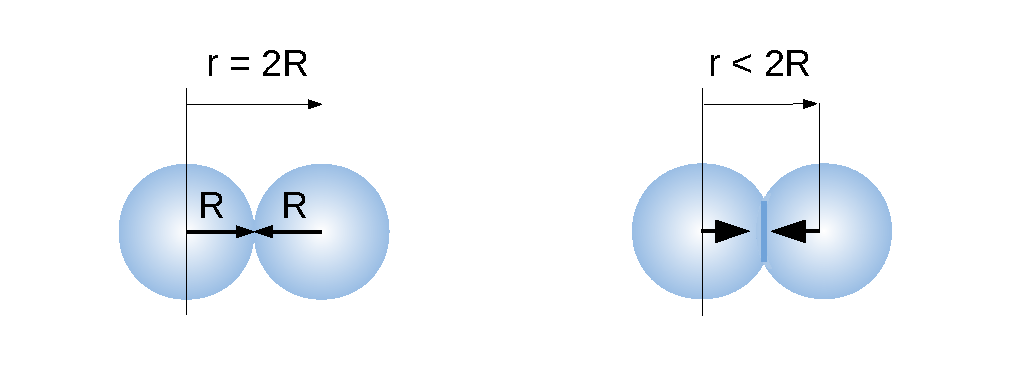
\includegraphics[width=0.8\columnwidth]{figs/TwoSpheres}
\end{frame}

\section*{Next section}
\begin{frame}{What is free energy?}
	\begin{block}{Intuitive}
			$F$ - the available work in the system
	\end{block}
    \begin{block}{Mathematics}
		\vspace{1em}
		\begin{columns}[t]
		\column{.5\textwidth}		
		{\centering Thermodynamics:
		\begin{align*}
			\diff F &= - S\,  \diff T + P\, \diff V
		\end{align*}}
		\column{.5\textwidth}
		{\centering
		Statistical Mechanics
		\begin{align*}
		F &= - k_B T \ln Z
		\end{align*}}
		\end{columns}
    \end{block}		
		Why Helmholtz and not Gibbs?
	\begin{itemize}
		\item Control temperature and volume 
		\item Entropy a more preferable partial derivative
	\end{itemize}
\end{frame}

\subsubsection*{Excess}
\begin{frame}{Excess free energy}	
	\begin{columns}[t]
	\setlength\abovedisplayskip{-2pt} 
	\column{.4\textwidth}	
	\begin{align*}
		Z_{exc} &= \int_s \frac{\diff\mathbf{r}^N}{V^N} ~e^{-\beta \Phi(\mathbf{r_1}, \mathbf{r_2}, \dots \mathbf{r_N})}
	\end{align*}
	\begin{itemize}
		\item No algebraic expression for even simple $\Phi$
		\item Need to use models, simulations to approximate behavior
		\item Even with models...
	\end{itemize}
	\column{.6\textwidth}
	\begin{figure}
		\caption{Hard sphere and square well intermolecular pair potentials.}
	\end{figure}
	\end{columns}
\end{frame}


\subsection*{Methods}
\begin{frame}{Methods}
	\begin{itemize}
		\item Thermodynamic Integration: integration over densities
		\item Square Well Monte Carlo: integration over temperature
	\end{itemize}
\end{frame}

\subsection*{Results}
\begin{frame}{Results}
\begin{columns}
	\column{.7\textwidth}
        FIXME the file figs/Fabs-vs-eta is missing
	%% \frame{\includegraphics[width=\textwidth]{figs/Fabs-vs-eta}}
	\column{.4\textwidth}
	\begin{itemize}
		\item Two doubling regimes simulated
		\item Becomes more negative with increasing temperature, density 
	\end{itemize}
\end{columns}
\end{frame}

\section*{Final thoughts}
\subsection*{Remarks}
\begin{frame}{Remarks}
	\begin{itemize}
		\item Liquids - however simple - are very complicated
		\item Simplest models have no analytic solutions
		\item Separation enables some behavioral investigation
	\end{itemize}
\end{frame}
\subsection*{References}
\begin{frame}{References}
	\tiny
	\begin{itemize}
		\item Retrieved from \url{https://nicokrisch.files.wordpress.com/2014/05/}
		\item Retrieved from \url{https://en.wikipedia.org/wiki/Chemical_polarity}
		\item I. M. J.-P. Hansen, Theory of Simple Liquids, $3^{\text{rd}}$ ed. (Academic Press, 2006).
		\item M. A. Perlin, ``Optimizing monte carlo simulation of the square-well fluid,'' (2015), Oregon State University.
		\item A. Valeske, ``Determining free energies of hard sphere fluids via monte carlo simulation'' (2015), Oregon State University.
	\end{itemize}
\end{frame}

\end{document}
